\documentclass[a4paper,10pt]{article}
\usepackage[utf8]{inputenc}
\usepackage{amsmath}
\usepackage{tabularx}
\usepackage{graphicx}
\usepackage{epstopdf}
\usepackage{textcomp}
\usepackage{amsmath}

\usepackage{listings}             % Include the listings-package


\newcolumntype{b}{X}
\newcolumntype{s}{>{\hsize=.25\hsize}X}

%opening
\title{Informe técnico: Adquisición de señales analógicas}
\author{P. Domenichini, A. Mendez}

\begin{document}

\maketitle

% Objetivos de mínima
% 1. Buscar y elegir una librería para control de la placa de audio.
% 2. Caracterizar la entrada de la placa de audio.
% 3. Caracterizar la salida de la placa de audio.
% 4. Reemplazar en el programa del día anterior el generador de
%    funciones o el osciloscopio por la placa de audio.
% 5. Curva de respuesta: Diodo, BJT o JFET
% 6. Implementar un circuito aplicando OPAMP o Regulador LM317
% 7. Armar una hoja de datos para reportar resultados

% Lineamientos
% I Formato tipo informe técnico
% I Detalles más relevantes del programa (diagrama de flujo, pseudocódigo, etc)
% I Descripción experimental
% I Especificar el programa utilizado para cada medición (si corresponde...)
% I Resumen de resultados tipo “hoja de datos”

\section{Placa de audio}
La adquisición de señales analógicas mediante control de placa 
de audio del presente trabajo se realizo a través de la utilización
de la librería {\sc pyaudio}. La caracterización de entrada y 
salida de la placa de audio utilizada está dada por la 
tabla~\ref{tab:inout-audio}.

\begin{table}[h]
\begin{tabularx}{\textwidth}{b|s|s|s }
Característica & Min & Max & Unidad \\
\hline
Voltaje señal de entrada & & & V \\ 
Voltaje señal de salida & & & V \\
Frecuencia señal de entrada & & & Hz \\
Frecuencia señal de salida & & & Hz \\
\end{tabularx}
\label{tab:inout-audio}
\caption{Caracterización de señales de entrada y salida de placa 
de audio.}
\end{table}

\subsection{Emisión y adquisición de señal con python}

La emisión y adquisición de señales mediante el uso de la placa
de audio se realizo con dos programas independientes de lectura y
escritura. Por ejemplo, el código de lectura que nos permitió 
adquirir las señales relevantes de los circuitos implementados en 
las secciones \ref{sec:diodo} y \ref{sec:opamp} tiene una estructura
similar al siguiente código:

\lstset{language=Python}
\begin{lstlisting}[frame=single]  % Start your code-block

import pyaudio
import numpy as np
p = pyaudio.PyAudio()
ftype=pyaudio.paInt16
nbuff=44100
stream = p.open(format=ftype,channels=1,
                rate=nbuff,input=True)
data = stream.read(nbuff)
stream.stop_stream()
stream.close()
p.terminate()
audioin_data = np.fromstring(data, np.int16)
\end{lstlisting}
% 
% \lstset{language=Python}
% \begin{lstlisting}[frame=single]  % Start your code-block
% 
% import pyaudio
% import numpy as np
% def sine(freq):
%    xfreq=int(nbuff/freq)
%    ntimes=int(duration*xfreq)
%    x=np.arange(xfreq*ntimes)
%    out=amp*np.sin(2*np.pi*x/xfreq)
%    return out.astype(np.float32)
% ftype=pyaudio.paFloat32
% nbuff=44100       # float32 sampling rate, Hz (int)
% duration=10.0      # in seconds
% amp=2**8/2        # wave amplitude
% volume=1.0        # range [0.0, 1.0] * amp
% freq=10000.0       # sine frequency, Hz
% samples=sine(freq)
% p = pyaudio.PyAudio()
% stream=p.open(format=ftype,channels=1,
%               rate=nbuff,output=True)
% stream.write(volume*samples)
% stream.stop_stream()
% stream.close()
% p.terminate()
% \end{lstlisting}

\section{Determinación de curva de respuesta de diodo}
\label{sec:diodo}

El circuito utilizado para determinar la curva de respuesta de
un diodo se muestra en la Figura~\ref{fig:diodo}a. Los diferencias
de tensión sobre el diodo y la resistencia fueron obtenidas
mediante el uso de la placa de audio. La curva I-V de respuesta
del diodo se muestra en la Figura~\ref{fig:diodo}b.

\begin{figure}
 \centering
 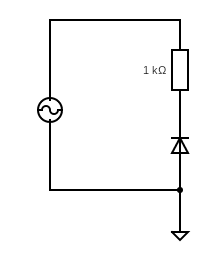
\includegraphics[trim={0 0 1cm 0},clip, width=0.3\textwidth]{circuit.png} (a)
 \hspace{0.1cm}
 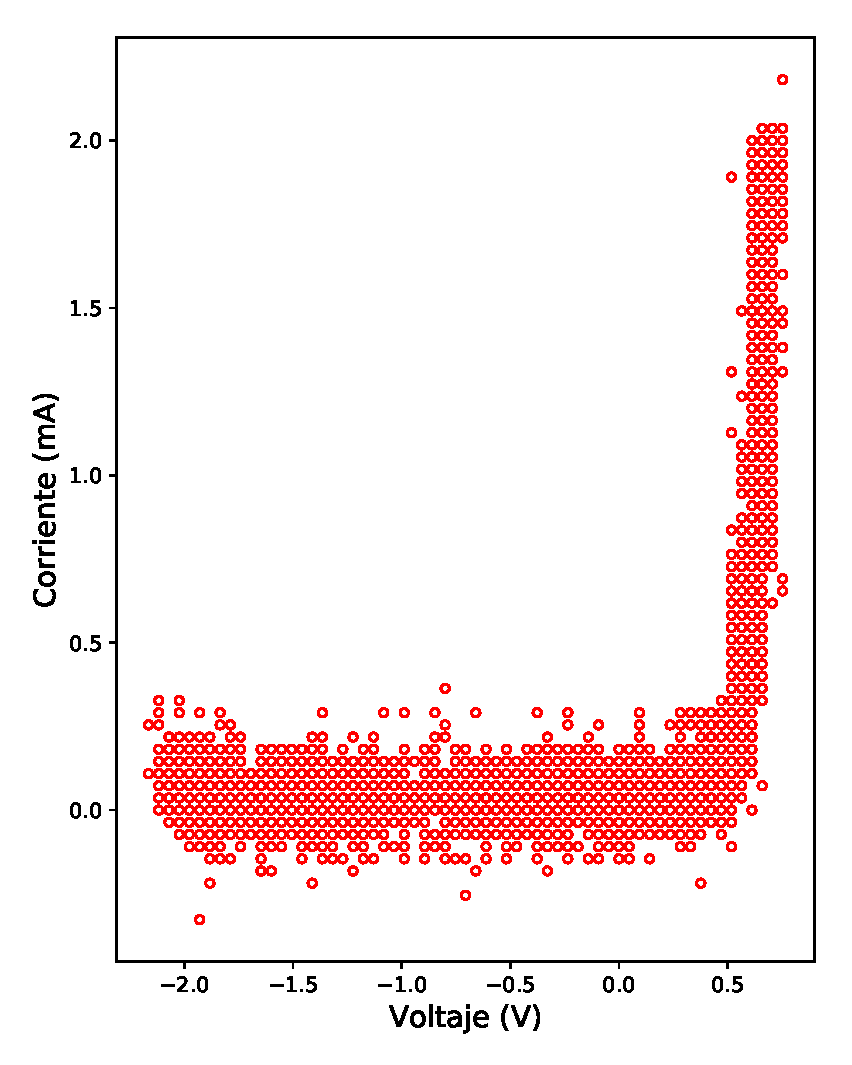
\includegraphics[width=0.35\textwidth]{diodo.eps} (b)
 \label{fig:diodo}
 \caption{(a) Esquema del circuito implementado. (b) Curva I-V del diodo.}
\end{figure}


\section{Implementación de OPAMP}
\label{sec:opamp}

\end{document}
